\documentclass{beamer}
\usepackage{HECbeamer}
% \usepackage{pgfpages}
% \pgfpagesuselayout{4 on 1}[letterpaper, landscape, border shrink=5mm]
\title[\color{white}{MATH 60604A \S~7b - Likelihood for survival analysis}]{\texorpdfstring{MATH 60604A \\Statistical modelling \\ \S~7b - Likelihood for survival analysis}{MATH 60604A \\Statistical modelling \\ \S~7b - Likelihood for survival analysis}}
\author{}
\institute{HEC Montréal\\
Department of Decision Sciences}
\date{} 

\begin{document}
\frame{\titlepage}



\begin{frame}
\frametitle{Survival and hazard functions} 

Let $T$ denote the survival time
\bi %\item On dénote la fonction de répartition $F(t) = \P{T \leq t}$ et la fonction de densité $f(t) = \d F(t) / \d t$. 
\item  The \alert{survival function}, $S(t) = \P{T>t}$, completely caracterizes the law of  $T$.
\item Often, we are more interested in knowing what time periods are characterized by higher failure rates.
The \alert{hazard}  of $T$ is
\begin{align*}
h(t) &= \lim_{\delta \to 0} \frac{\P{t < T<t + \delta \mid T>t}}{\delta} 
\\&= \lim_{\delta \to 0} \frac{1}{\delta}\frac{\P{t < T < t + \delta}}{\P{T>t}} \\&= \frac{f(t)}{S(t)}
\end{align*}
We can think of the hazard rate as being the instantaneous probability of ``dying'' at time $t$, given survival to time $t$.
\ei
\end{frame}
\begin{frame}[fragile]
\frametitle{Survival function and hazard function}
\begin{center}
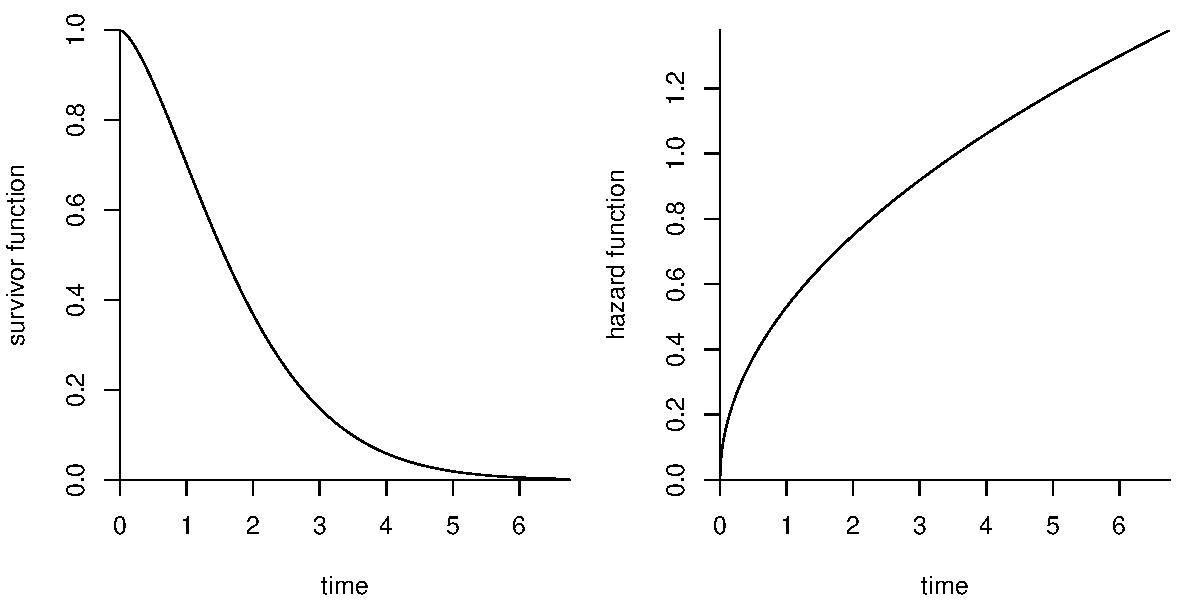
\includegraphics[width = 0.8\textwidth]{img/c7/07-survival-hazard.pdf}
\end{center}
{\footnotesize

The survival function decreases monotically from $S(0)=1$. The higher the hazard $h(t)$, the fastest the decrease of the survival function.

}

\end{frame}

\begin{frame}
\frametitle{Bathtub shaped hazard}
\begin{center}
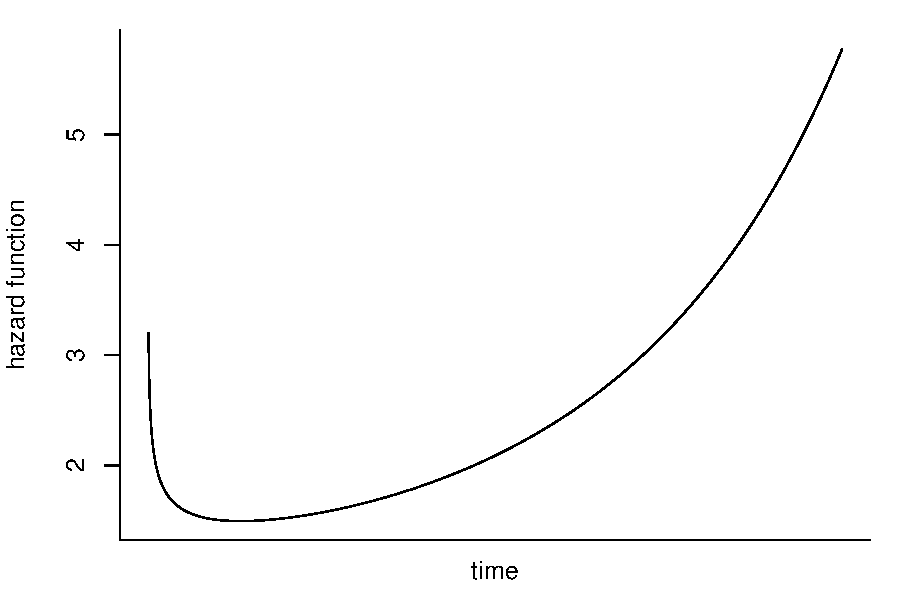
\includegraphics[width = 0.8\textwidth]{img/c7/07-bathtub-hazard.pdf}
\end{center}
{\footnotesize
Typical hazard shape: the risk rate is high (e.g., childhood mortality, manufacturing defect) initially, then decreases and plateau. As time goes on, the hazard increases steadily.

}
\end{frame}

\begin{frame}
\frametitle{Random censoring and likelihood}
We observe $T_i = \min\{T_i^0, C_i\}$. If an observation is right-censored at time $c$, we know that $S(c)=\P{T_i^0 > c}$
\bi \item in other words, survival time exceeds $c$.
\ei

If we have censoring, the database includes an indicator variable $\delta_i$ where
\begin{align*}
T_i = 
\begin{cases}
T_i^0, & \delta_i=1 \text{ (observed failure time)}\\
C_i, & \delta_i=0 \text{ (right-censored)}
\end{cases}
\end{align*}
\end{frame}


\begin{frame}
\frametitle{Likelihood contribution}
Let $S(t; \bs{\theta}) = \P{T_{i}^0 > t}$ denote the survival function of $T_i^0$. If $T_i^0$ is independent of $C_i$, the likelihood contribution of each observation is
\begin{align*}
L_i(\bs{\theta}) = 
\begin{cases} 
f(t_i; \bs{\theta}), & \delta_i=1 \text{ (observed failure time)}\\
S(t_i; \bs{\theta}), & \delta_i=0 \text{ (right-censored)}
\end{cases}.
\end{align*}
We can therefore write the log likelihood as
\begin{align*}
\ell(\bs{\theta}) \equiv \sum_{i: \delta_i=1} \ln f(t_i; \bs{\theta}) + \sum_{i: \delta_i=0} \ln S(t_i; \bs{\theta})
\end{align*}

\end{frame}
\begin{frame}
\frametitle{Inferential approaches}

Many avenues are open for estimating the survival function (or hazard).
\bi \item parametric: choose a family of distributions (Weibull, log normal, Gompertz, exponential) for $T$.
\bi
\item[$+$] can easily incorporate explanatories
\item[$+$] continuous function, can be used to extrapolate
\item[$-$] subject to model misspecificiation
\item[$-$] not flexible: can fit poorly to the data.
\ei
\item nonparametric: no distributional assumption
\bi 
\item[$-$] no explanatory variable
\item[$+$] minimal hypotheses, theoretical guarantees for large sample size
\item[$+$] flexible
\item[$-$] yields discontinuous estimates
\item[$-$] cannot extrapolate beyond the largest observed time.
\ei
\ei
\end{frame}


\begin{frame}
\frametitle{Parametric model for survival: exponential distribution}
Consider $T_i \simiid \mathsf{E}(\lambda)$, i.e., exponential variables with expectation $\lambda^{-1}$.
\bi \item 
The survival function of  $T$ is $S(T) = \exp(-\lambda t)$ and
\item the hazard $h(t)=\lambda$ is \textbf{constant}.
\ei
The log likelihood for a random sample of size $n$ is
\begin{align*}
\ell(\lambda) =\sum_{i=1}^n \{\delta_i \ln \lambda - \lambda T_i\}.
\end{align*}
The maximum likelihood estimator is $\widehat{\lambda} =\sum_{i=1}^n \delta_i/ \sum_{i=1}^n T_i $. 

\bi \item The estimated survival time is infinite if no one failed.
\item The standard errors are obtained from the observed information matrix $j(\widehat{\lambda}) = \sum_{i=1}^n \delta_i/\widehat{\lambda}^2$; censored observations contribute no information.
\ei

\end{frame}
\end{document}
